% !TEX root = ../master-thesis.tex


The ability to prepare arbitrary atom configurations is a key ingredient for bottom-up quantum simulation. After obtaining unit filling for both spin states (as discussed in Sec.~\ref{subsec:balancing} and \ref{subsec:spin-selective-spilling}), a multi-stage spilling sequence can be implemented that enables spin- and site-resolved initialization of arbitrary patterns. This approach with additional spilling stages was developed in this work and represents a step towards arbitrary pattern preparation for 2D fermions, which has not been previously demonstrated. While the theoretical framework and initial experimental validation are presented here, full implementation of arbitrary pattern preparation awaits the installation of an additional microwave antenna for complete spin control between states $\ket{1}$ and $\ket{2}$, which is currently in progress. The loading sequence proceeds in several steps:
\begin{enumerate*}
    \item Prepare a $\ket{1}$–$\ket{2}$ spin mixture with unit filling across the tweezer array.
    \item Perform global spilling steps to remove atoms from factorized intensity patterns $P_{ij}$, affecting both spin states.
    \item Apply spin-selective spilling steps to remove atoms in state $\ket{1}$ from additional factorized subsets of sites.
    \item Flip the remaining atoms $\ket{1} \leftrightarrow \ket{2}$ using a microwave $\pi$-pulse (currently in progress).
    \item Repeat spin-selective spilling to further refine the configuration
\end{enumerate*}

% \textbf{Factorized removal.}
Each spilling step removes atoms from sites where the local tweezer depth $P_{ij}$ falls below a certain threshold. Since any rank-1 intensity mask $P_{ij} = H_i V_j$ can be imposed, it is possible to tailor the removal region to arbitrary product forms. To remove a single atom at site $(i', j')$, for example, $H_{i'}$ and $V_{j'}$ are reduced by a factor $\eta < 1$ while simultaneously increasing the global power by $\eta$. This yields a relative intensity of $1/\eta$ at the intersection, while leaving all other sites unchanged or increased in depth. In this way, atoms can be reliably isolated and removed from any desired factorized subset.

% \textbf{Boolean decomposition.}
The cumulative removal pattern can be represented as a binary matrix $W_{ij}$, where $W_{ij} = 1$ indicates that the atom at site $(i, j)$ has been removed. Each spilling operation adds a binary outer product $u^\lambda_i v^\lambda_j$ via Boolean logic ($1 + 1 = 1$). An arbitrary target pattern can therefore be reached through a sequence of such operations:
\begin{equation}
    \label{eq:ebmf}
    W_{ij} = \bigvee_{\lambda=1}^{r} u^\lambda_i v^\lambda_j,
\end{equation}
which defines the exact Boolean matrix factorization (EBMF) of the removal matrix. In the worst case, any binary $n \times n$ matrix admits such a decomposition using at most $n$ steps.

% \textbf{Optimal EBMF.}
While a naive strategy (such as row- or column-wise removal) may require up to $n$ iterations, optimal EBMF often reduces this number. The problem of finding an exact Boolean matrix factorization with minimal rank is known to be NP-complete~\cite{orlin_contentment_1977} and NP-hard to approximate~\cite{gruber_inapproximability_2007}. Nevertheless, for arrays up to $10 \times 10$, optimal decompositions can be computed in a few seconds using a SAT solver. These improvements are particularly useful for minimizing experimental cycle time and improving overall sequence fidelity. A full discussion of the EBMF algorithm and its implementation is presented in Sec. \ref{subsec:bmfsat}.

% \textbf{Experimental performance and limitations.}
In this work, no reduction in preparation fidelity from additional spilling stages was observed. With sufficient intensity reduction $\eta < 0.5$, there is substantial margin in trap depth, making additional spilling stages significantly easier to implement than the initial doublon preparation spilling. The primary limitation is the finite lifetime of atoms in the tweezers. Each additional spilling stage currently requires approximately 20 ms (without optimization, further investigation into timing limits remains open). For an arbitrary configuration in an $N \times N$ array, at most $N$ additional spilling stages per spin state are required, corresponding to a maximum of $2N$ total stages. For a $10 \times 10$ array, this amounts to 400 ms in the current implementation. Given the characteristic tweezer lifetime of 17 s (at 1.3 mW tweezer power), this yields an estimated fidelity of 95\% for $10 \times 10$ arrays based purely on lifetime considerations in the worst-case scenario. For $6 \times 6$ arrays, the fidelity reaches 98.6\%. For the measurements shown in Fig.~\ref{fig:spillingadd}, only 3 additional spilling stages were used, resulting in no observable impact on the overall experimental fidelity. Here, fidelity refers to the probability of detecting a doublon (two particles) at the intended site, consistent with the definition used throughout this work.

Sequential additional spilling stages could potentially be avoided using a Digital Micromirror Device (DMD), which is currently being installed in the experimental setup. With a DMD, specific potentials can be applied during spin-selective spilling such that atoms are selectively spilled from desired lattice sites, enabling parallel pattern preparation. Implementation via DMD remains a future direction for this work.

\begin{figure}
    \centering
    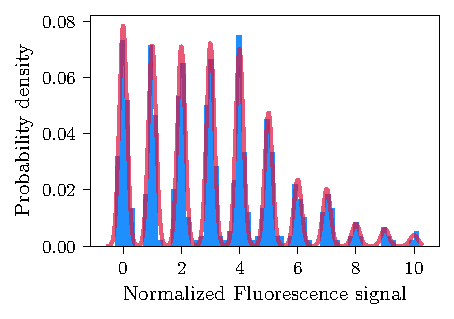
\includegraphics{fig-py/atom-counting.pdf}
    \caption[Single atom counting]{
        \textbf{Single atom counting.}
        Calibration histogram for single-atom counting based on fluorescence signal after loading to the MOT. Clear quantized peaks correspond to integer atom numbers; the solid red line is a multi-Gaussian fit to the distribution. 
    }
    \label{fig:spillingadd}
\end{figure}